\documentclass[tikz,border=7pt]{standalone}
\usepackage{amssymb}
\usepackage{pgfplots}
\pgfplotsset{compat=1.18}
\begin{document}
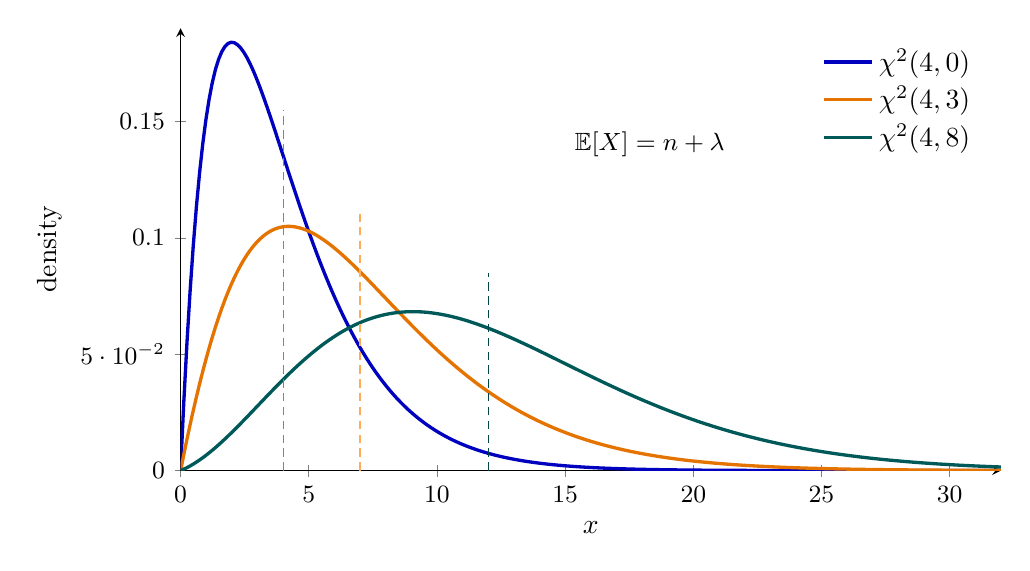
\begin{tikzpicture}
\begin{axis}[
  width=12cm,
  height=7.2cm,
  axis lines=left,
  xmin=0,
  xmax=32,
  ymin=0,
  ymax=0.19,
  samples=260,
  xlabel={$x$},
  ylabel={density},
  legend style={draw=none,fill=white,at={(0.98,0.98)},anchor=north east},
  tick label style={font=\small}
]
% For n=4, use the Poisson-mixture representation
% exp(-(x+lambda)/2) sum_k lambda^k x^(k+1)/(2^(2k+2) k! (k+1)!).
\addplot[blue!75!black,very thick,domain=0.001:32]
  {exp(-x/2)*x/4};
\addlegendentry{$\chi^2(4,0)$}

\addplot[orange!90!black,very thick,domain=0.001:32]
  {exp(-(x+3)/2)*(
    x/4 + 3*x^2/32 + 9*x^3/768 + 27*x^4/36864
    + 81*x^5/2949120 + 243*x^6/353894400
    + 729*x^7/59454259200 + 2187*x^8/13317754060800
    + 6561*x^9/3835513169510400)};
\addlegendentry{$\chi^2(4,3)$}

\addplot[teal!70!black,very thick,domain=0.001:32]
  {exp(-(x+8)/2)*(
    x/4 + 8*x^2/32 + 64*x^3/768 + 512*x^4/36864
    + 4096*x^5/2949120 + 32768*x^6/353894400
    + 262144*x^7/59454259200 + 2097152*x^8/13317754060800
    + 16777216*x^9/3835513169510400
    + 134217728*x^10/1380784741023744000)};
\addlegendentry{$\chi^2(4,8)$}

\draw[densely dashed,blue!55] (axis cs:4,0) -- (axis cs:4,0.155);
\draw[densely dashed,orange!65] (axis cs:7,0) -- (axis cs:7,0.11);
\draw[densely dashed,teal!55!black] (axis cs:12,0) -- (axis cs:12,0.085);
\node[font=\small,anchor=west] at (axis cs:15,0.14)
  {$\mathbb{E}[X]=n+\lambda$};
\end{axis}
\end{tikzpicture}
\end{document}
